\chapter{O$_2$ Module}

The O$_2$ module is a simple oxygen evolution module,
intermediate between the Street and Phelps
\cite{kashefipour_dispersion_2002} type of model,
which is restricted to modeling reaeration and the global oxidizable load,
and a more complete module, such as EUTRO, which simulates several oxidation processes
and explicitly shows the evolution of phytoplankton and its influence on oxygen.
The O$_2$ model’s advantage is its simplicity
(eight parameters to calibrate, excluding parameterization of weirs).
Some important parameters are taken as constant such as benthic demand or plant respiration.
The use of the model is consequently limited to phenomena of a few days duration,
such as emptying of a reservoir. Three tracers are involved:

\begin{itemize}
\item dissolved oxygen O$_2$ (mgO$_2$/l),
\item the organic load L (mgO$_2$/l),
\item the ammonia load NH4 (mgO$_2$/l).
\end{itemize}

These variables are carried and dispersed in the mass of water and their evolution
conforms accordingly to the advection-dispersion equation,
with external and internal sources.
Six factors influencing the concentration of dissolved oxygen are considered:

\begin{itemize}
\item four factors that consume oxygen: organic load, ammonia load,
  benthic demand and plant respiration,
\item two processes that create oxygen: photosynthesis and reaeration.
\end{itemize}

The terms dealing with internal sources of each considered tracer are explained
in the following paragraphs.

\section{Dissolved oxygen}

\subsection{Benthic demand}

Benthic demand $BEN$ is provided by the user. It is expressed in gO$_2$/m$^2$/d.
It is adjusted for temperature $T$ according to the relation:

\begin{equation}
  BEN_T = BEN_{20^\circ \rm{C}} (1.065)^{T-20}.
\end{equation}

The following Table gives some typical values of benthic demand.\\

\begin{table}[H]
 			\centering
\begin{tabular}{p{3.0in}p{3.0in}}
\hline
%row no:1
\multicolumn{1}{|p{3.0in}}{Bottom type} & 
\multicolumn{1}{|p{3.0in}|}{Typical value of $BEN$ (g/m$^2$/d) at 20$^{\circ}$C} \\
\hline
%\hhline{--}
%row no:2
\multicolumn{1}{|p{3.0in}}{Filamentous bacteria (10~g/m$^2$)} & 
\multicolumn{1}{|p{3.0in}|}{7} \\
\hline
%\hhline{--}
%row no:3
\multicolumn{1}{|p{3.0in}}{Mud from waste water, near to discharge} & 
\multicolumn{1}{|p{3.0in}|}{4} \\
\hline
%\hhline{--}
%row no:4
\multicolumn{1}{|p{3.0in}}{Mud from waste water, far from discharge } & 
\multicolumn{1}{|p{3.0in}|}{1.5} \\
\hline
%\hhline{--}
%row no:5
\multicolumn{1}{|p{3.0in}}{Estuarine silt} & 
\multicolumn{1}{|p{3.0in}|}{1.5} \\
\hline
%\hhline{--}
%row no:6
\multicolumn{1}{|p{3.0in}}{Sandy bottom} & 
\multicolumn{1}{|p{3.0in}|}{0.5} \\
\hline
%\hhline{--}
%row no:7
\multicolumn{1}{|p{3.0in}}{Mineral soil} & 
\multicolumn{1}{|p{3.0in}|}{0.007} \\
\hline
%\hhline{--}

\end{tabular}
\end{table}

\subsection{Plant respiration}

Plant respiration $R$ (in mgO$_2$/d/l) is provided by the user.

\subsection{Photosynthesis}

Photosynthesis $P$ (in mgO$_2$/d/l) depends on algae, water depth and light.
Its order of magnitude is between 0.3 mgO$_2$/l/d and 9 mgO$_2$/l/d
depending on the water flow \cite{streeter_ohio_1925}.
In the O$_2$ model, it is provided by the user.

\subsection{Reaeration}

\subsubsection{Natural reaeration}

Reaeration is an oxygen supply through the free surface.
At macroscopic scale, it can be modeled as a rate proportional to ($C_s$ - [O$_2$]),
where $C_s$ is the oxygen concentration at saturation in the water (in mgO$_2$/l)
(Reminder: $C_s$ = 9 mg/l at 20$^{\circ}$C). Therefore:

\begin{equation}
  Reaeration = k_2 \left( C_s - [\rm{O}_2] \right).
\end{equation}

The coefficient $k_2$ (d$^{-1}$) is a parameter of the model.
Its orders of magnitude are indicated in the Table below
(from \cite{tchobanoglous_wq_1985}).\\

\begin{table}[H]
 			\centering
\begin{tabular}{p{3.0in}p{3.0in}}
\hline
%row no:1
\multicolumn{1}{|p{3.0in}}{Type of watercourse} & 
\multicolumn{1}{|p{3.0in}|}{Interval of $k_2$ (d$^{-1}$) at 20$^{\circ}$C} \\
\hline
%\hhline{--}
%row no:2
\multicolumn{1}{|p{3.0in}}{Small ponds and backwaters} & 
\multicolumn{1}{|p{3.0in}|}{0.10-0.23} \\
\hline
%\hhline{--}
%row no:3
\multicolumn{1}{|p{3.0in}}{Sluggish streams and large lakes} & 
\multicolumn{1}{|p{3.0in}|}{0.23-0.35} \\
\hline
%\hhline{--}
%row no:4
\multicolumn{1}{|p{3.0in}}{Large streams of low velocity} & 
\multicolumn{1}{|p{3.0in}|}{0.35-0.46} \\
\hline
%\hhline{--}
%row no:5
\multicolumn{1}{|p{3.0in}}{Large streams of normal velocity} & 
\multicolumn{1}{|p{3.0in}|}{0.46-0.69} \\
\hline
%\hhline{--}
%row no:6
\multicolumn{1}{|p{3.0in}}{Swift streams} & 
\multicolumn{1}{|p{3.0in}|}{0.69-1.15} \\
\hline
%\hhline{--}
%row no:7
\multicolumn{1}{|p{3.0in}}{Rapids and waterfalls} & 
\multicolumn{1}{|p{3.0in}|}{> 1.15} \\
\hline
%\hhline{--}

\end{tabular}
\end{table}

There are a large number of formulae for calculating $k_2$,
which indicates the low level of understanding this process.
We can distinguish between conceptual formulae,
valid only within conditions allowed by the hypotheses,
and semi-empirical and empirical formulae,
that are valid where conditions are not too far from those of calibration.
In reality, there is little difference between the formulae when water depth
is between 0.3 and 3 m.
The O$_2$ model allows us to use four formulae cited in \cite{mccutcheon_wq_1989}:

\begin{equation}
  k_2 = 5.23 U h^{-1.67} \quad \rm{(Tennessee~Valley~Authority)},
\end{equation}

\begin{equation}
  k_2 = 5.33 U^{0.67} h^{-1.85} \quad \rm{(Owens~et~al.)},
\end{equation}

\begin{equation}
  k_2 = 0.746 U^{2.695} h^{-3.085} J^{-0.823} \quad \rm{(Churchill~et~al.)},
\end{equation}

\begin{equation}
  k_2 = 3.9 U^{0.5} h^{-1.5} \quad \rm{(O’Connor~and~Dobbins)}.
\end{equation}

The O’Connor and Dobbins formula seems to provide the best results for shallow rivers.
For deep and rapid rivers, that of Churchill et al. is preferable.
The diagram shows the areas of application for each of three formulae \cite{mccutcheon_wq_1989}:

\begin{figure}[H]
  \centering
  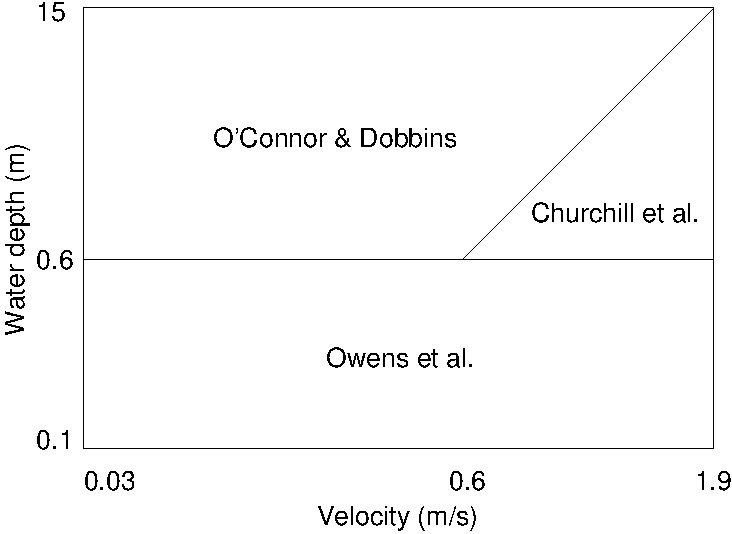
\includegraphics[scale=0.3]{graphics/validity_domain_reaeration_O2.png}
  \caption{Application areas of Owens et al., Churchill et al. and O'Connor
    and Dobbins formulae \cite{mccutcheon_wq_1989}.}
\end{figure}

One option in the model allows the use of a fixed value for $k_2$, chosen by the user,
another allows choosing one of the four formulae described above.
The value of $k_2$, valid at 20$^{\circ}$C, is adjusted to temperature according to the following formula:

\begin{equation}
  k_2 = (k_2)_{20^{\circ}\rm{C}} (1.0241)^{T-20}.
\end{equation}

Oxygen concentration at saturation in the water $C_s$ can be determined
by the water temperature (at 20$^{\circ}$C, $C_s$ = 9 mg/l).
This becomes a parameter that must be known and can itself be calculated
if connected to a temperature model such as THERMIC.
Elmore and Hayes (cited in \cite{mccutcheon_wq_1989}) give the following formula
(with $T$ in $^{\circ}$C) for calculating $C_s$:

\begin{equation}
  C_s = 14.652 - 0.41022 T + 0.007991 T^2 - 7.7774.10^{-5}T^3.
\end{equation}

More recent models include a correction for atmospheric pressure and, in estuaries, for salinity.
However, we consider that we are far from estuarial conditions and the variations in pressure
entail insignificant variations in dissolved oxygen compared to those that we need.
The following equation of Montgomery et al. (cited in \cite{mccutcheon_wq_1989})
only deviates from standard formulae by $ \pm $  0.02 mg/l
between 0 and 50$^{\circ}$C when there is negligible salinity.

\begin{equation}
  C_s = \frac{468}{31.6+T}.
\end{equation}

The model allows us to choose either a fixed value for $C_s$ given
by the user or one of the two formulae described above.\\

\subsubsection{Reaeration due to weirs (not used at the moment in WAQTEL)}

A weir can provide between 1 and 3 mg/l of dissolved oxygen \cite{mccutcheon_wq_1989}.
We define $r$ by the relationship $$r = \frac{C_s-C_u}{C_s-C_d},$$

with $C_u$ = concentration upstream of weir, $C_d$ = concentration downstream of weir.
The knowledge of $C_u$ and $r$  enables us to calculate $C_d$.
In this model, $C_d$ is directly applied from this formula.
This term therefore is not treated as a source.
The rate $r$ can be determined with the aid of formulae in the literature
\cite{mccutcheon_wq_1989}: e.g.,

\begin{equation}
  r = 1 + 0.5 a b \Delta h \quad \rm{(Gameson)},
\end{equation}

\begin{equation}
  r = 0.11 a b (1+0.046 T) \Delta h \quad \rm{(Gameson~et~al.)},
\end{equation}

\begin{equation}
  r = 1 + 0.69 \Delta h (1 - 0.11 \Delta h) (1 +0.046 T) \quad \rm{(Water~Research~Laboratory)},
\end{equation}

\begin{equation}
  r = 1 + 0.38 a b  \Delta h (1 - 0.11 \Delta h) (1 +0.046 T),
  \quad \rm{(Water~Research~Laboratory)}
\end{equation}

with $a$ = measure of water quality (= 0.65 for grossly polluted strams,
= 1.8 for clear streams),
$b$ = characteristic parameter of weir type,
$\Delta h$ = water level difference between upstream and downstream.
The following Table gives the $b$ values for different types of weir (according to \cite{mccutcheon_wq_1989}):\\

\begin{table}[H]
 			\centering
\begin{tabular}{p{3.0in}p{3.0in}}
\hline
%row no:1
\multicolumn{1}{|p{3.0in}}{Type of weir} & 
\multicolumn{1}{|p{3.0in}|}{$b$} \\
\hline
%\hhline{--}
%row no:2
\multicolumn{1}{|p{3.0in}}{flat broad-crested regular step} & 
\multicolumn{1}{|p{3.0in}|}{0.7} \\
\hline
%\hhline{--}
%row no:3
\multicolumn{1}{|p{3.0in}}{flat broad-crested irregular step} & 
\multicolumn{1}{|p{3.0in}|}{0.8} \\
\hline
%\hhline{--}
%row no:4
\multicolumn{1}{|p{3.0in}}{flat broad-crested vertical face} & 
\multicolumn{1}{|p{3.0in}|}{0.8} \\
\hline
%\hhline{--}
%row no:5
\multicolumn{1}{|p{3.0in}}{flat broad-crested straight slope face} & 
\multicolumn{1}{|p{3.0in}|}{0.9} \\
\hline
%\hhline{--}
%row no:6
\multicolumn{1}{|p{3.0in}}{flat broad-crested curved face} & 
\multicolumn{1}{|p{3.0in}|}{0.75} \\
\hline
%\hhline{--}
%row no:7
\multicolumn{1}{|p{3.0in}}{round broad-crested curved face} & 
\multicolumn{1}{|p{3.0in}|}{0.6} \\
\hline
%\hhline{--}
%row no:8
\multicolumn{1}{|p{3.0in}}{sharp-crested straight slope face} & 
\multicolumn{1}{|p{3.0in}|}{1.05} \\
\hline
%\hhline{--}
%row no:9
\multicolumn{1}{|p{3.0in}}{sharp-crested vertical face} & 
\multicolumn{1}{|p{3.0in}|}{0.8} \\
\hline
%\hhline{--}
%row no:10
\multicolumn{1}{|p{3.0in}}{sluice gates with submerged discharge} & 
\multicolumn{1}{|p{3.0in}|}{0.05} \\
\hline
%\hhline{--}

\end{tabular}
\end{table}

In the model, $r$ can be either a fixed value given by the user or
one of the 4 formulae previously described.\\

\section{Organic load}

The organic load $L$ (in mgO$_2$/l) is a variable evolving over time
from an initial condition according to a law that is assumed to be 1$^{\rm{st}}$ order:

\begin{equation}
  F([L]) = -k_1 [L],
\end{equation}

where $k_1$ is the constant of kinetic degradation of the organic load (d$^{-1}$).
It is a parameter of the model.
In the O$_2$ model, the organic load is considered to be an independent variable.

\section{Ammonia load}

Also consuming oxygen, the variable ammonia load NH$_4$ (in mgO$_2$/l) also follows
a 1$^{\rm{st}}$ order law of decay

\begin{equation}
  F([NH_4]) = -k_4 [NH_4],
\end{equation}

where $k_4$ is the kinetic constant of nitrification (d$^{-1}$),
a parameter of the model.
In the O$_2$ model, the ammonia load is considered to be an independent variable.\\

\section{Solved equation}

The concentration of dissolved oxygen [O$_2$] (in mgO$_2$/l) changes
through the effect of sources, written as follows:

\begin{equation}
  F([O_2]) = k_2 (C_s - [O_2]) -k_1 [L] - k_4 [NH_4] + P - R - \frac{BEN_T}{h}.
\end{equation}

In this way, using the terminology and notations of section \ref{waq_models}
and setting $C_1$ = [O$_2$], $C_2$ = [L] and $C_3$ = [NH$_4$],
the matrices [$ \lambda $] and [$ \mu $] containing the coefficients
$\lambda_i^j$ and $ \mu_i^j$ are written as:\\

$$  [\lambda] = \frac{1}{86400}
  \begin{pmatrix}
    -k_2 & -k_1  & -k_4 \\
     0   & -k_1  & 0    \\
     0   &  0    & -k_4
  \end{pmatrix}
$$
  
$$
  [\mu] = 
  \begin{pmatrix}
     0  & 0_2 & 0 \\
     0  & 0   & 0 \\
     0  & 0   & 0
  \end{pmatrix}
$$  

(Note: Division by 86,400 scales down the time to one second).\\

The only non-zeros terms $ \lambda_1^0$ and $ \mu_1^0$ are:

\begin{equation}
  \lambda_1^0 = \frac{k_2 C_s + P - R}{86400},
\end{equation}

\begin{equation}
  \mu_1^0 = -\frac{BEN_T}{86400}.
\end{equation}
